% GRASP: Copyright 1997,1998,1999  Bruce Allen
% $Id: man_ringdown.tex,v 1.9 1999/09/29 00:23:29 ballen Exp $
\section{GRASP Routines: Black hole ringdown}

Stellar-sized black hole binaries are an important source of gravitational
radiation for ground-based interferometric detectors.  The radiation arises
from three phases: the inspiral of the two black hole companions, the merger
of these two companions to form a single black hole, and the ringdown of this
initially distorted black hole to become a stationary Kerr black hole.
The gravitational radiation of the black hole inspiral has been discussed
in section~\ref{s:inspiral}; calculations of the late stages of inspiral, the
merger, and the early stages of the ringdown have not yet been completed;
the radiation produced in the late stages of black hole ringdown is the topic
of this section.

At late times, the distorted black hole will be sufficiently ``similar to''
a stationary Kerr black hole that the distortion can be expanded in terms
of ``resonant modes'' of the Kerr black hole.  By ``resonant modes'' we refer
to the eigenfunctions of the Teukolsky equation---which describes linear
perturbations of the Kerr spacetime---with boundary conditions corresponding to
purely ingoing radiation at the event horizon and purely outgoing radiation
at large distances.  These resonant modes are also called the quasinormal
modes; they are described in the next subsection.


\clearpage
\subsection{Quasinormal modes of black holes}
\label{ss:Quasimodo}
Gravitational perturbations of the curvature of Kerr black holes can be
described by two components of the Weyl tensor: $\Psi_0$ and~$\Psi_4$.
Because these are components of the curvature tensor, they have dimensions
of $[L^{-2}]$.
Of particular interest is the quantity~$\Psi_4$ since it is this term that is
suitable for the study of outgoing waves in the radiative zone.  The
formalism for the study of perturbations of rotating black holes was
developed originally by Teukolsky~\cite{teukolsky:1973} who was able
to separate the differential equation to obtain solutions of the form
\begin{equation}
  (r-i\mu a)^4\Psi_4 = e^{-i\omega t} {}_{-2}R_{\ell m}(r)
                       {}_{-2}S_{\ell m}(\mu) e^{im\beta}
  \label{e:perturbation mode}
\end{equation}
where ${}_{-2}R_{\ell m}(r)$ is a solution to a radial differential
equation, and~${}_{-2}S_{\ell m}(\mu)$ is a spin-weighted spheroidal wave
function (see~\cite{teukolsky:1973}, equations (4.9) and~(4.10)).
The black hole has mass~$M$ and \emph{specific angular momentum}~$a=cJ/M$
(which has dimensions of length) where $J$ is the angular momentum of the
spinning black hole.  We shall often refer to the
\emph{dimensionless angular momentum parameter}, $\hat{a}=c^2a/GM=c^3J/GM^2$.
For a Kerr black hole, $\hat{a}$ must be between zero (Schwarzschild limit)
and one (extreme Kerr limit).
The observer of the perturbation is located at radius~$r$,
inclination~$\mu=\cos\iota$, and azimuth~$\beta$
(see figure~\ref{f:orient}).  The perturbation
itself has the spheroidal eigenvalues $\ell$ and~$m$, and has a
(complex) frequency~$\omega$.  The constants $G$ and~$c$ are Newton's
gravitational constant and the speed of light.

\begin{figure}[h]
\begin{center}
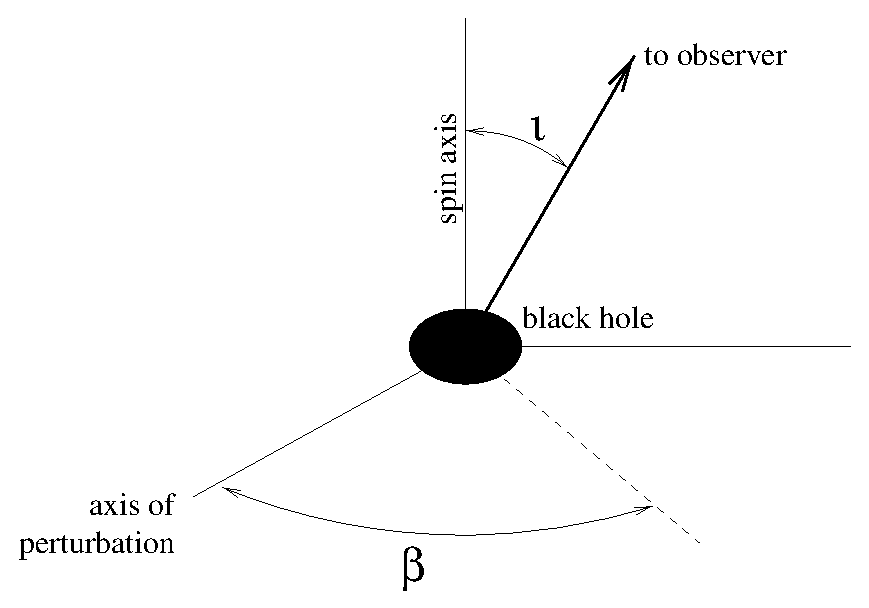
\epsfig{file=Figures/orient.eps,height=6cm}
\caption{\label{f:orient} The polar angle, $\iota$, and the azimuthal angle,
  $\beta$, of the observer relative to the spin axis of a black hole and
  the (somewhat arbitrary) axis of perturbation.}
\end{center}
\end{figure}

The important physical quantities for the study of the gravitational
waves arising from black hole perturbations can be recovered from the
field~$\Psi_4$.  In particular, the ``$+$'' and~``$\times$'' polarizations
of the strain induced by the gravity waves are found
by~\cite{teukolsky:1973}
\begin{equation}
  h_+ - ih_\times = -\frac{2c^2}{|\omega|^2}\,\Psi_4\;.
  \label{e:perturbation strain}
\end{equation}
The quantity~$h_+=h_{\hat\iota\hat\iota}$ is the metric perturbation
that represents the linear polarization state along
${\mathbf{e}}_{\hat\iota}$ and~${\mathbf{e}}_{\hat\beta}$, while the
quantity~$h_\times=h_{\hat\iota\hat\beta}$ represents the linear
polarization state
along~${\mathbf{e}}_{\hat\iota}\pm{\mathbf{e}}_{\hat\beta}$.  The power
radiated towards the observer (per unit solid angle) is
\begin{equation}
  \frac{d^2E}{dt\,d\Omega} = \lim_{r\to\infty}
  \frac{c^7r^2}{4\pi G|\omega|^2} \, |\Psi_4|^2\;.
  \label{e:perturbation power}
\end{equation}
Thus, in order to compute the relevant information about gravitational
waves emitted as perturbations to rotating black hole spacetimes, one
needs to calculate the value of~$\Psi_4$ at large radii from the black hole.

The quasinormal modes are resonant modes of the Teukolsky equation
that describe purely outgoing radiation in the wave-zone and purely
ingoing radiation at the event horizon.  The quasi-normal modes are
described by a spectrum of complex eigenvalues (which include the
spectrum of eigenfrequencies~$\omega_n$), and
eigenfunctions ${}_{-2}R_{\ell m}(r)$
and~${}_{-2}S_{\ell m}(\mu)$ for each value spheroidal mode $\ell$
and~$m$.  These eigenvalues and functions also depend on the mass and
angular momentum of the black hole.  We shall only consider
the fundamental ($n=0$) mode since the harmonics of this mode have
shorter lifetimes.  For the same reason, we are most interested in the
quadrupole ($\ell=2$ and~$m=2$) mode.  The observer is assumed to be at a large
distance; in this case, one can approximate the perturbation as follows:
\begin{equation}
  \Psi_4 \approx \frac{A}{r}\,e^{-i\omega t_{\mathrm{\scriptscriptstyle ret}}}
    {}_{-2}S_{\ell m}(\mu)e^{im\beta}.
  \label{e:asymp perturbation}
\end{equation}
Here $t_{\mathrm{\scriptstyle ret}}=t-r^\star/c$ represents the retarded time,
where~$r^\star$ is a ``tortoise'' radial parameter.  For large radii, the
tortoise radius behaves as $r-r_+\log(r/r_+)$ where~$r_+$ is the ``radius''
of the black hole event horizon.  Thus, we see that the tortoise radius is
nearly equal to the distance of the objects surrounding the black hole,
and we shall view it as the ``distance to the black hole.''  The
parameter~$A$ represents the amplitude of the perturbation, which has the
dimensions of~$[L^{-1}]$.

Given the asymptotic form of the perturbation in
equation~\ref{e:asymp perturbation}, we can integrate
equation~\ref{e:perturbation power} over the entire sphere and the
interval~$t_{\mathrm{\scriptstyle ret}}\in[0,\infty)$ to obtain an expression
for the total energy
radiated in terms of the amplitude~$A$ of the perturbation.  Thus, we can
characterize the amplitude by the total amount of energy emitted:
$A^2=4Gc^{-7}E|\omega|^2(-{\mathrm{Im}}\,\omega)$.  The gravitational waveform
is found to be
\begin{equation}
  h_+ - ih_\times \approx - \frac{4c}{r}
    \biggl(\frac{-{\mathrm{Im}}\,\omega}{|\omega|^2}\biggr)^{1/2}
    \biggl(\frac{GE}{c^5}\biggr)^{1/2}
    e^{-i\omega t_{\mathrm{\scriptscriptstyle ret}}}
    {}_{-2}S_{\ell m}(\mu) e^{im\beta}.
  \label{e:quasinormal ring strain}
\end{equation}
In order to simulate the quasinormal ringing of a black hole, it is necessary
to determine the complex eigenvalues of the desired mode,
and then to compute the spheroidal wave function~$S_{\ell m}(\mu)$.  The
routines to perform these computations are discussed in the following sections.

Rather than computing the actual gravitational strain waveforms at the
detector, the routines will calculate the quantity
$H_+-iH_\times=(c^2r/GM_\odot)(h_+-ih_\times)$; the normalization
of these waveforms to the correct source distance is left to the calling
routine.  The distance normalization can be computed as follows:
\begin{equation}
  \frac{c^2r}{GM_\odot} = \frac{r}{T_\odot c}
    = \biggl( \frac{r}{1.4766\,{\mathrm{km}}} \biggr)
    = 2.090\times10^{19}\biggl( \frac{r}{\mathrm{Mpc}} \biggr).
  \label{e:radius in solar masses}
\end{equation}
where $T_\odot=4.925491\,\mu{\mathrm{s}}$ is the mass of the sun expressed in
seconds (see equation~\ref{e:tsolar}).
It will be convenient to write the time dependence of the strain as the
complex function~${\mathcal{H}}(t_{\mathrm{\scriptstyle ret}})$ so that
$H_+-iH_\times={\mathcal{H}}(t_{\mathrm{\scriptstyle ret}})
 {}_{-2}S_{\ell m}(\mu)e^{im\beta}$.
The dimensionless eigenfrequency, $\hat{\omega}=GM\omega/c^3$,
depends only on the mode and the dimensionless
angular momentum of the black hole.  In terms of this quantity,
the function~${\mathcal{H}}(t_{\mathrm{\scriptstyle ret}})$ is
\begin{equation}
  {\mathcal{H}}(t_{\mathrm{\scriptstyle ret}}) \approx -4 \epsilon^{1/2}
    \frac{(-{\mathrm{Im}}\,\hat{\omega})^{1/2}}{|\hat{\omega}|}
    \biggl(\frac{M}{M_\odot}\biggr)
    \exp\biggl[-i\hat{\omega}\biggl(
      \frac{t_{\mathrm{\scriptstyle ret}}}{T_\odot}\biggr)
      \biggl(\frac{M}{M_\odot}\biggr)^{-1}\biggr]
  \label{e:dimensionless strain function}
\end{equation}
where $\epsilon$ is the fractional mass loss due to the radiation in the
excited quasinormal mode.


\clearpage
\subsection{Function: \texttt{qn\_eigenvalues()}}
\label{ss:qn_eigenvalues}

\begin{verbatim}
void qn_eigenvalues(float eigenvalues[], float a, int s, int l, int m)
\end{verbatim}
This routine computes the eigenvalues associated with the spheroidal and
radial wave functions for a specified quasinormal mode.  The arguments are:
\begin{description}
\item{\texttt{eigenvalues}}: Output.  An array, \texttt{eigenvalues[0..3]},
  which contains, on output, the real and imaginary parts of the eigenvalues
  $\hat{\omega}$ and~$A$ (see below) as follows:
  $\texttt{eigenvalues[0]}={\mathrm{Re}}\,\hat{\omega}$,
  $\texttt{eigenvalues[1]}={\mathrm{Im}}\,\hat{\omega}$,
  $\texttt{eigenvalues[2]}={\mathrm{Re}}\,A$,
  and~$\texttt{eigenvalues[3]}={\mathrm{Im}}\,A$.
\item{\texttt{a}}: Input.  The dimensionless angular momentum parameter
  of the Kerr black hole, $|\hat{a}|\le1$, which is negative if the black hole
  is spinning clockwise about the~$\iota=0$ axis (see figure~\ref{f:orient}).
\item{\texttt{s}}: Input.  The integer-valued spin-weight~$s$, which should
  be set to $0$~for a scalar perturbation (e.g., a scalar field perturbation),
  $\pm1$~for a vector perturbation (e.g., an electromagnetic field
  perturbation), or $\pm2$ for a spin two perturbation (e.g., a gravitational
  perturbation).
\item{\texttt{l}}: Input.  The mode integer~$\texttt{l}\ge|\texttt{s}|$.
\item{\texttt{m}}: Input.  The mode integer~$|\texttt{m}|\le\texttt{l}$.
\end{description}

For a Kerr black hole of a given dimensionless angular momentum parameter,
$\hat{a}$, with a
perturbation of spin-weight~$s$ and mode $\ell$ and~$m$, there is a spectrum
of quasinormal modes which are specified by the eigenvalues $\hat{\omega}_n$
and~$A_n$.  As discussed in the previous subsection, the
eigenvalue~$\hat{\omega}_n$ is associated with the separation of the time
dependence of the perturbation, and it specifies the frequency and damping
time of the radiation from the perturbation.  The additional complex
eigenvalue~$A_n$ results from the separation of the radial and azimuthal
dependence into the spheroidal and radial wave functions.  Both of these
eigenvalues will be necessary for the computation of the spheroidal wave
function (below).

The routine \texttt{qn\_eigenvalues()} can be used to compute the eigenvalues
of the fundamental ($n=0$) mode.  To convert the dimensionless eigenvalue
$\hat{\omega}$ to the (complex) frequency of the ringdown of a Kerr black
hole of mass~$M$, one simply computes~$\omega=c^3\hat{\omega}/GM$.
The eigenfrequency is computed using the method of Leaver~\cite{leaver:1985}.
Note that Leaver adopts units in which~$2M=1$, so one finds that
$\hat{\omega}=\frac{1}{2}\omega_{\mathrm{\scriptscriptstyle Leaver}}$ and
$\hat{a}=2a_{\mathrm{\scriptscriptstyle Leaver}}$ in our notation.
The eigenvalues satisfy the following symmetry: if $\rho_m=-i\hat{\omega}_m$
and~$A_m$ are the eigenvalues for an azimuthal index~$m$, then
$\rho_{-m}=\rho_m^\ast$ and~$A_{-m}=A_m^\ast$ are the eigenvalues for the
azimuthal index~$-m$.

\begin{description}
\item{Author:} Jolien Creighton, jolien@tapir.caltech.edu
\item{Comment:} For simplicity, we require that the spin-weight
number, $s$, be an integer.  Thus, the spinor perturbations $\chi_0$
and~$\chi_1$, associated with $s=\pm\frac{1}{2}$
respectively~\cite{teukolsky:1973}, are not allowed.
\end{description}


\clearpage
\subsection{Example: \texttt{eigenvalues} program}

This example uses the function \texttt{qn\_eigenvalues()} to compute the
eigenvalues ${}_s\hat{\omega}_{\ell m}$ and~${}_sA_{\ell m}$ for the
$s$~spin-weighted quasinormal mode specified by $\ell$ and~$m$, and for
a range of values of the dimensionless angular momentum parameter, $\hat{a}$.
To invoke the program, type:
\begin{quote}
\texttt{eigenvalues} $s$ $\ell$ $m$
\end{quote}
for the desired (integer) values of $s$, $\ell$, and~$m$.  Make sure that
$\ell\ge|s|$ and~$0\le m\le\ell$ (the eigenvalues for negative values of
$m$ can be inferred from the symmetries discussed in
subsection~\ref{ss:qn_eigenvalues}).  The output of the program is five
columns of data: the first column is the value of~$\hat{a}$ running from just
greater than~$-1$ to just less than~$1$ (or between $0$ and~$1$ if $m=0$),
the second and third columns are the real and imaginary parts of the
eigenfrequency~$\hat{\omega}$, and the fourth and fifth columns are the
real and imaginary parts of the angular separation eigenvalue~$A$.
For the values of~$\hat{a}<0$, the eigenvalues correspond to the mode
with azimuthal index~$-m$ so that the real part of the eigenfrequency is
positive.  A plot of the eigenfrequency output of the program
\texttt{eigenvalues} for several runs with~$s=-2$ is shown in
figure~\ref{f:eigen}.  The blue curves in figure~\ref{f:eigen} can be compared
to figure~5 of reference~\cite{onozawa:1997} keeping in mind the conversion
factors between Leaver's convention (which is also used in~\cite{onozawa:1997})
and the convention used here (see subsection~\ref{ss:qn_eigenvalues}).

\begin{figure}[h]
\index{colorpage}
\begin{center}
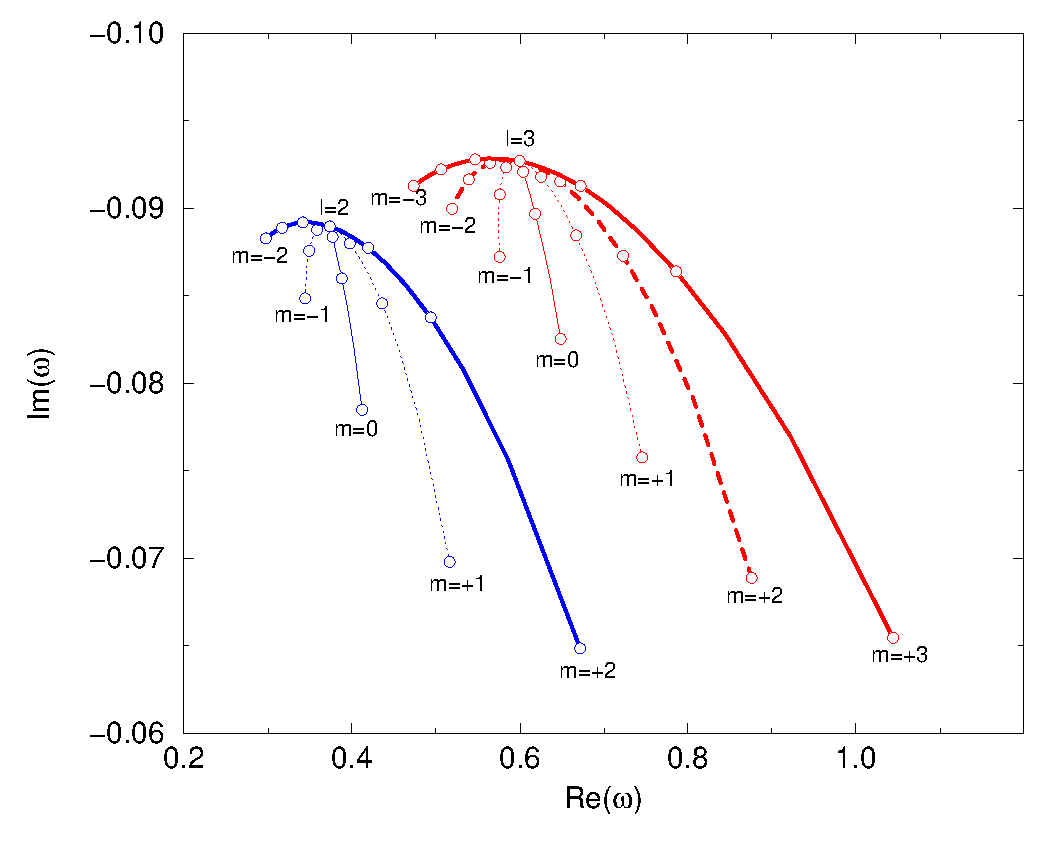
\epsfig{file=Figures/eigen.eps,height=7.5cm}
\caption{\label{f:eigen} The real and imaginary parts of the eigenfrequencies,
  $\hat{\omega}$, as computed by the program \texttt{eigenvalues} with $s=-2$.
  Each curve corresponds to a range of values of $\hat{a}$ from $-0.9$ (left)
  to~$+0.9$ (right) for a single mode $\ell$ and $|m|$.  The open circles are
  placed at the values $\hat{a}=-0.9$, $-0.6$, $-0.3$, $0$, $+0.3$, $+0.6$,
  and~$+0.9$ except when $m=0$ in which case there are no negative values
  of~$\hat{a}$ plotted.  The blue curves correspond to the $\ell=2$ modes and
  the red curves correspond to the $\ell=3$ modes.}
\end{center}
\end{figure}

\clearpage
\lgrindfile{Includes/eigenvalues.tex}

\begin{description}
\item{Author:} Jolien Creighton, jolien@tapir.caltech.edu
\end{description}


\clearpage
\subsection{Function: \texttt{sw\_spheroid()}}
\label{ss:sw_spheroid}

\begin{verbatim}
void sw_spheroid(float *re, float *im, float mu, int reset,
                 float a, int s, int l, int m, float eigenvalues[])
\end{verbatim}
This routine computes the spin-weighted spheroidal wave
function~${}_sS_{\ell m}(\mu)$.  The arguments are:
\begin{description}
\item{\texttt{re}}: Output.  The real part of the spin-weighted spheroidal
  wave function.
\item{\texttt{im}}: Output.  The imaginary part of the spin-weighted spheroidal
  wave function.
\item{\texttt{mu}}: Input.  The independent variable, $\mu=\cos\iota$ with
  $\iota$ being a polar angle, of the spin-weighted spheroidal wave function;
  $-1<\texttt{mu}<1$.
\item{\texttt{reset}}: Input.  A flag that indicates that the function should
  reset ($\texttt{reset}=1$) the internally stored normalization of the
  spin-weighted spheroidal wave function.  The reset flag should be set
  if any of the following five arguments are changed between calls; otherwise,
  set $\texttt{reset}=0$ so that the routine does not recompute the
  normalization.
\item{\texttt{a}}: Input.  The dimensionless angular momentum parameter,
  $-1<\texttt{a}<1$, of the Kerr black hole for which the spin-weighted
  spheroidal wave function is associated.
\item{\texttt{s}}: Input.  The integer-valued spin-weight~$s$, which should
  be set to $0$~for a scalar perturbation (e.g., a scalar field perturbation),
  $\pm1$~for a vector perturbation (e.g., an electromagnetic field
  perturbation), or $\pm2$ for a spin two perturbation (e.g., a gravitational
  perturbation).
\item{\texttt{l}}: Input.  The mode integer~$\texttt{l}\ge|\texttt{s}|$.
\item{\texttt{m}}: Input.  The mode integer~$|\texttt{m}|\le\texttt{l}$.
\item{\texttt{eigenvalues}}: Input.  An array, \texttt{eigenvalues[0..3]},
  which contains the real and imaginary parts of the eigenvalues
  $\hat{\omega}$ and~$A$ (see below) as follows:
  $\texttt{eigenvalues[0]}={\mathrm{Re}}\,\hat{\omega}$,
  $\texttt{eigenvalues[1]}={\mathrm{Im}}\,\hat{\omega}$,
  $\texttt{eigenvalues[2]}={\mathrm{Re}}\,A$,
  and~$\texttt{eigenvalues[3]}={\mathrm{Im}}\,A$.  These may be calculated for
  a quasinormal mode using the routine \texttt{qn\_eigenvalues()}.
\end{description}

The spin-weighted spheroidal wave function
is also computed using the method of Leaver~\cite{leaver:1985}.
We have adopted the following normalization criteria for the spin-weighted
spheroidal wave functions~${}_sS_{\ell m}(\mu)$.  First, the angle-averaged
value of the squared modulus of~${}_sS_{\ell m}(\mu)$ is unity:
$\int_{-1}^{1}|{}_sS_{\ell m}(\mu)|^2d\mu=1$.  Second, the complex phase is
partially fixed by the requirement that ${}_sS_{\ell m}(0)$ is real.
Finally, the sign is set to be $(-)^{\ell-\max(m,s)}$ for the real part
in the limit that
$\mu\to-1$ in order to agree with the sign of the spin-weighted spherical
harmonics~${}_sY_{\ell m}(\mu,0)$ (see~\cite{goldberg:1967}).

It is sufficient to compute the spin-weighted spheroidal wave functions
with $s<0$ and~$a\omega=\hat{a}\hat{\omega}\ge0$ because of the following
symmetries~\cite{press:1973}:
\begin{equation}
  {}_{-s}S_{\ell m}(\mu,a\omega) = {}_sS_{\ell m}(-\mu,a\omega)
  \quad {\textrm{with}} \quad
  {}_{-s}E_{\ell m}(a\omega) = {}_sE_{\ell m}(a\omega)
\end{equation}
and
\begin{equation}
  {}_sS_{\ell m}(\mu,-a\omega) = {}_sS_{\ell,-m}(-\mu,a\omega)
  \quad {\textrm{with}} \quad
  {}_sE_{\ell m}(-a\omega) = {}_sE_{\ell,-m}(a\omega)
\end{equation}
where ${}_sE_{\ell m}={}_sA_{\ell m}+s(s+1)$.

\begin{description}
\item{Author:} Jolien Creighton, jolien@tapir.caltech.edu
\end{description}


\clearpage
\subsection{Example: \texttt{spherical} program}

The program \texttt{spherical} is an example implementation of the
routine \texttt{sw\_spheroid()} to compute the standard spin-weighted
spherical harmonics~\cite{goldberg:1967}.  The program also computes these
functions using equation~(3.1) of~\cite{goldberg:1967} for comparison.
According to the normalization convention stated in
subsection~\ref{ss:sw_spheroid}, the relationship between the spin-weighted
spheroidal harmonics and the spin-weighted spherical harmonics is:
\begin{equation}
  {}_sY_{\ell m}(\theta,\phi) =
    (2\pi)^{-1/2}{}_sS_{\ell m}(\cos\theta)e^{im\phi}
\end{equation}
with $a\omega=0$ and~$A=(\ell-s)(\ell+s+1)$.

To invoke the program, type:
\begin{quote}
  \texttt{spherical} $s$ $\ell$ $m$
\end{quote}
for the desired (integer) values of $s$, $\ell$, and~$m$
($\ell\ge|s|$ and~$|m|\le\ell$).  The output is three columns of data: the
first column is the independent variable~$\mu$ between $-1$ and~$+1$, the
second column is the value of~$(2\pi)^{-1/2}{}_sS_{\ell m}(\mu)$, and the
third column is the value of~${}_sY_{\ell m}(\mu,0)$ as computed from
equation~(3.1) of~\cite{goldberg:1967}.  A comparison of the results produced
by the program \texttt{spherical} for $\ell=m=-s=2$ with the exact values
of ${}_{-2}Y_{22}(\mu,0)=(5/64\pi)^{1/2}(1+\mu)^2$ is shown in
table~\ref{t:spherical harmonic}.

\begin{table}[h]
\begin{center}
\begin{tabular}{|cccc|}
  \hline
  $\mu$ & Goldberg & \texttt{sw\_spheroid()} & exact \\
  \hline\hline
  $-0.99$ & $1.576955\times10^{-5}$ & $1.576955\times10^{-5}$ 
          & $1.576958\times10^{-5}$ \\
  $-0.95$ & $3.942387\times10^{-4}$ & $3.942387\times10^{-4}$
          & $3.942395\times10^{-4}$ \\
  $-0.75$ & $9.855968\times10^{-3}$ & $9.855967\times10^{-3}$
          & $9.855986\times10^{-3}$ \\
  $-0.55$ & $3.193334\times10^{-2}$ & $3.193333\times10^{-2}$
          & $3.193340\times10^{-2}$ \\
  $-0.35$ & $6.662639\times10^{-2}$ & $6.662639\times10^{-2}$
          & $6.663647\times10^{-2}$ \\
  $-0.15$ & $1.139351\times10^{-1}$ & $1.139351\times10^{-1}$
          & $1.139352\times10^{-1}$ \\
  $+0.15$ & $2.085525\times10^{-1}$ & $2.085525\times10^{-1}$
          & $2.085527\times10^{-1}$ \\
  $+0.35$ & $2.874004\times10^{-1}$ & $2.874005\times10^{-1}$
          & $2.874006\times10^{-1}$ \\
  $+0.55$ & $3.788640\times10^{-1}$ & $3.788639\times10^{-1}$
          & $3.788641\times10^{-1}$ \\
  $+0.75$ & $4.829430\times10^{-1}$ & $4.829430\times10^{-1}$
          & $4.829433\times10^{-1}$ \\
  $+0.95$ & $5.996378\times10^{-1}$ & $5.996379\times10^{-1}$
          & $5.996382\times10^{-1}$ \\
  $+0.99$ & $6.244906\times10^{-1}$ & $6.244906\times10^{-1}$
          & $6.244911\times10^{-1}$ \\
  \hline
\end{tabular}
\end{center}
\caption{\label{t:spherical harmonic}
  A comparison of the values of the spin-weighted spherical harmonic
  ${}_{-2}Y_{22}(\mu,0)$ calculated by equation~(3.1) of
  Goldberg~\protect\cite{goldberg:1967}, the values of
  $(2\pi)^{-1/2}{}_{-2}S_{22}(\mu)$ using routine \texttt{sw\_spheroid()},
  and the values of the exact result $(5/64\pi)^{1/2}(1+\mu)^2$.  The three
  methods give excellent agreement.}
\end{table}

\clearpage
\lgrindfile{Includes/spherical.tex}

\begin{description}
\item{Author:} Jolien Creighton, jolien@tapir.caltech.edu
\end{description}


\clearpage
\subsection{Example: \texttt{spheroid} program}

This is a second implementation of the function \texttt{sw\_spheroid()}
which is used to compute the spin-weighted spheroidal wave function
associated with a quasinormal ringdown mode of a Kerr black hole with
a certain (specified in the code) dimensionless angular momentum parameter.  
To invoke the program, type:
\begin{quote}
  \texttt{spheroid} $s$ $\ell$ $m$
\end{quote}
for the desired (integer) values of $s$, $\ell$, and~$m$
($\ell\ge|s|$ and~$|m|\le\ell$) of the desired mode.
The output is three columns of data: the
first column is the independent variable~$\mu$ between $-1$ and~$+1$, the
second column is the value of the real part of~${}_sS_{\ell m}(\mu)$, and the
third column is the value of the imaginary part of~${}_sS_{\ell m}(\mu)$.
Figure~\ref{f:spheroid} depicts the output for the spin-weighted spheroidal
wave function~${}_{-2}S_{22}(\mu)$.

\begin{figure}[h]
\begin{center}
\index{colorpage}
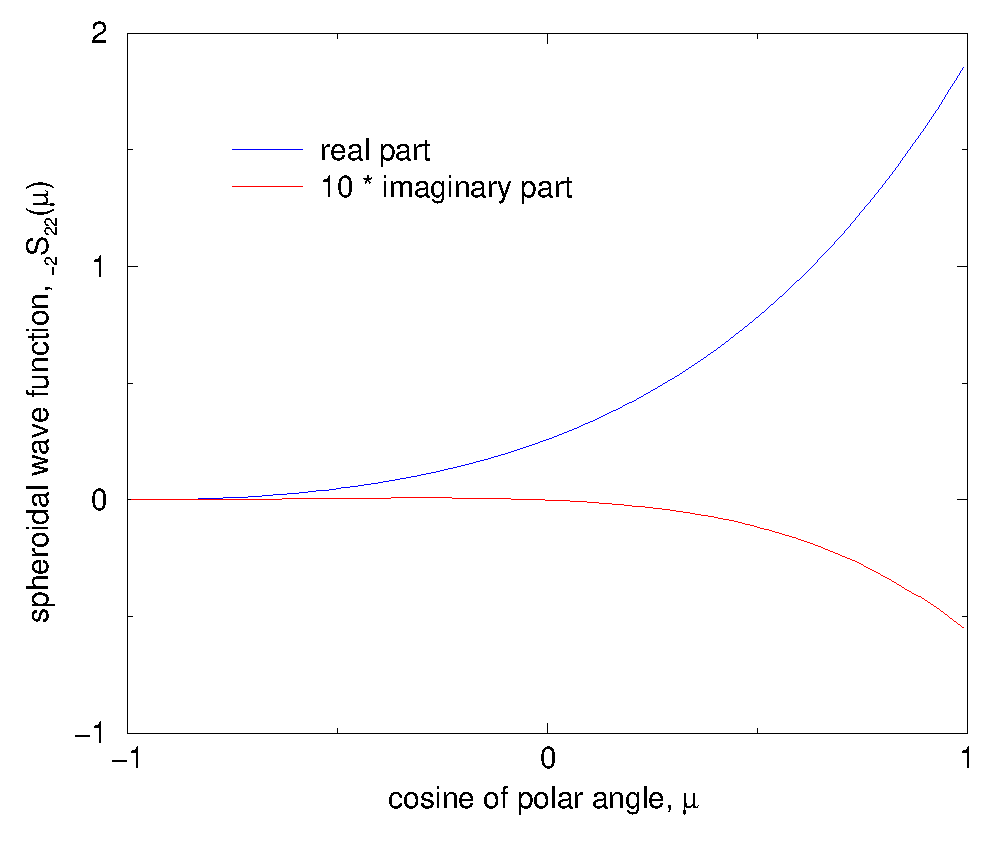
\epsfig{file=Figures/spheroid.eps,height=7.5cm}
\caption{\label{f:spheroid} A plot of the real and imaginary parts of the
  $\ell=m=-s=2$ spin-weighted spheroidal wave function, ${}_{-2}S_{22}(\mu)$,
  associated with a black hole with dimensionless angular momentum
  parameter~$\hat{a}=0.98$.  The imaginary part is scaled by a factor of ten.}
\end{center}
\end{figure}

\clearpage
\lgrindfile{Includes/spheroid.tex}

\begin{description}
\item{Author:} Jolien Creighton, jolien@tapir.caltech.edu
\end{description}


\clearpage
\subsection{Function: \texttt{qn\_ring()}}

\begin{verbatim}
int qn_ring(float iota, float beta,
            float eps, float M, float a, int l, int m,
            float dt, float atten, int max,
            float **plusPtr, float **crossPtr)
\end{verbatim}
This routine is used to compute the ``$+$'' and~``$\times$'' polarizations
of the gravitational waveform, $H(t_{\mathrm{\scriptstyle ret}})$, produced by
a black hole ringdown at a distance
$GM_\odot/c^2=T_\odot c\simeq1.4766\,{\mathrm{km}}$.  To obtain the waveforms
at a distance~$r$, multiply the result by $GM_\odot/c^2r=T_\odot c/r$.
The arguments are:
\begin{description}
\item{\texttt{iota}}: Input.  The polar angle (inclination), $\iota$
  (in radians), of
  the sky position of the observer with respect to the (positive) spin axis
  of the black hole, $0\le\texttt{iota}\le\pi$.
\item{\texttt{beta}}: Input.  The azimuth, $\beta$ (in radians),
  of the sky position
  of the observer with respect to the axis of the perturbation at the start
  time.  ($0\le\texttt{beta}\le2\pi$.)
\item{\texttt{eps}}: Input.  The fraction of the total mass lost
  in gravitational radiation from the particular mode. ($0<\texttt{eps}\ll1$.)
\item{\texttt{M}}: Input.  The mass of the black hole in solar masses.
\item{\texttt{a}}: Input.  The dimensionless angular momentum parameter
  of the Kerr black hole, $|\hat{a}|\le1$, which is negative if the black hole
  is spinning clockwise about the~$\iota=0$ axis (see figure~\ref{f:orient}).
\item{\texttt{l}}: Input.  The mode integer $\ell$.  ($\texttt{l}\ge2$)
\item{\texttt{m}}: Input.  The mode integer $m$.  ($|\texttt{m}|\le\texttt{l}$)
\item{\texttt{dt}}: Input.  The time interval, in seconds, between successive
  data points in the returned waveforms.
\item{\texttt{atten}}: Input.  The attenuation level, in dB, at which the
  routine will terminate calculation of the waveforms.  I.e., the routine
  will terminate when the amplitude,
  $A=A_0\exp(-{\mathrm{Im}}\,\omega t_{\mathrm{\scriptstyle ret}})$, falls below
  the level~$A_{\mathrm{\scriptstyle cutoff}}=A_0\,{\mathrm{alog}}_{10}(-0.1\times
  \texttt{atten})$.
\item{\texttt{max}}: Input.  The maximum number of data points to be returned
  in the waveforms.
\item{\texttt{plusPtr}}: Input/Output.  A pointer to an array which, on
  return, contains the waveform~$H_+$ sampled at intervals \texttt{dt}.
  If the array has the value \texttt{NULL} on input, the routine allocates
  an amount of memory to \texttt{*plusPtr} to hold \texttt{max} elements.
\item{\texttt{crossPtr}}: Input/Output.  A pointer to an array which, on
  return, contains the waveform~$H_\times$ sampled at intervals \texttt{dt}.
  If the array has the value \texttt{NULL} on input, the routine allocates
  an amount of memory to \texttt{*crossPtr} to hold \texttt{max} elements.
\end{description}

The routine \texttt{qn\_ring()} returns the number of data points that were
written to the arrays \texttt{(*plusPtr)[]} and \texttt{(*crossPtr)[]}; this
is either the number specified by the input parameter \texttt{max} or the
number of points computed when the waveform was attenuated by the threshold
\texttt{atten}.  The eigenvalues are obtained from the function
\texttt{qn\_eigenvalues()}.  The waveform is
then computed using $H_+-iH_\times={\mathcal{H}}(t_{\mathrm{\scriptstyle ret}})
 {}_{-2}S_{\ell m}(\mu)e^{im\beta}$
with~${\mathcal{H}}(t_{\mathrm{\scriptstyle ret}})$ given by
equation~(\ref{e:dimensionless strain function}).  The spheroidal wave function
is obtained from the function \texttt{sw\_spheroid()}.

\begin{description}
\item{Author:} Jolien Creighton, jolien@tapir.caltech.edu
\end{description}


\clearpage
\subsection{Example: \texttt{ringdown} program}

This example uses the function \texttt{qn\_ring()} to compute the black hole
quasinormal ringdown waveform for a preset mode and inclination.  The waveform
as a function of time is written to standard output in three columns: the time,
the plus polarization, and the cross polarization.  A Plot of the quasinormal
ringdown waveform data is shown in figure~\ref{f:ring}.

\begin{figure}[h]
\begin{center}
\index{colorpage}
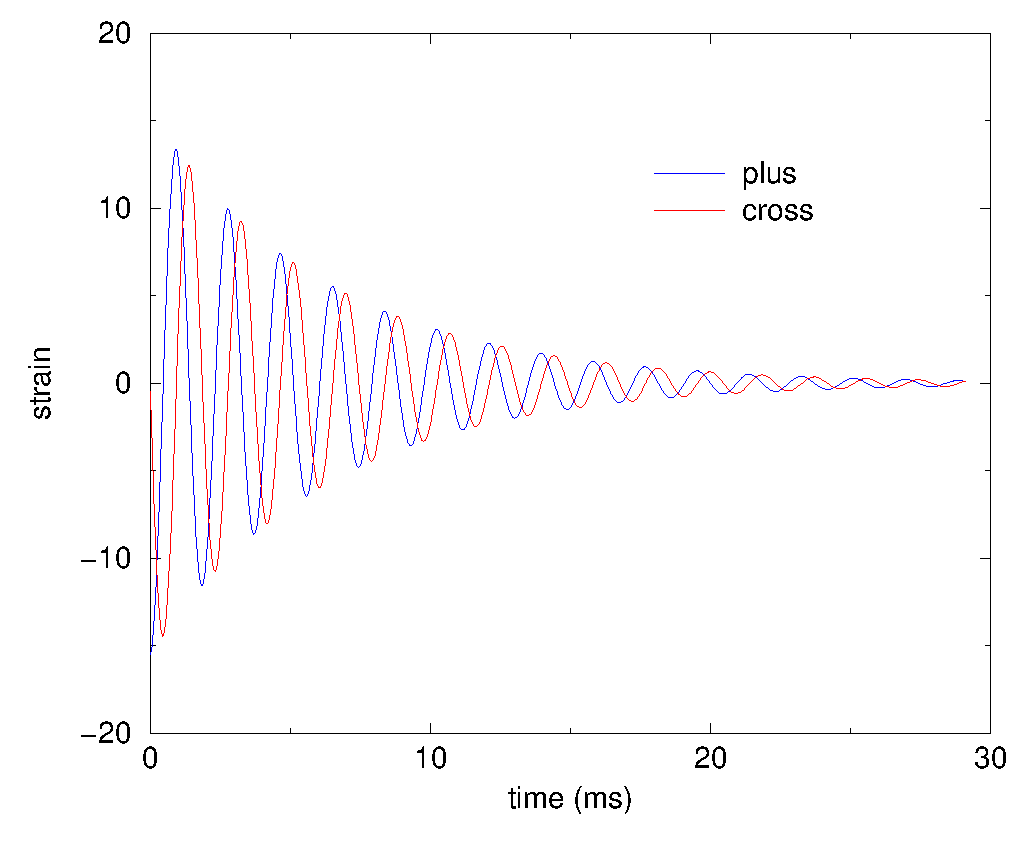
\epsfig{file=Figures/ring.eps,height=7.5cm}
\caption{\label{f:ring} A plot of the plus and cross polarizations of the
  gravitational wave strain, at a (unphysical!)
  distance~$GM_\odot/c^2=T_\odot c\simeq1.4766\,{\mathrm{km}}$,
  for the fundamental
  $\ell=m=2$ mode of a black hole with mass $M=50M_\odot$, dimensionless
  angular momentum parameter~$0.98$, and fractional mass loss $\epsilon=0.03$,
  with inclination and azimuth $\iota=0$ and~$\beta=0$.  The data was produced
  by the program \texttt{ringdown}.}
\end{center}
\end{figure}

\clearpage
\lgrindfile{Includes/ringdown.tex}

\begin{description}
\item{Author:} Jolien Creighton, jolien@tapir.caltech.edu
\end{description}


\clearpage
\subsection{Function: \texttt{qn\_qring()}}

\begin{verbatim}
int qn_qring(float psi0, float eps, float M, float a,
             float dt, float atten, int max, float **strainPtr)
\end{verbatim}
The routine \texttt{qn\_qring()} is a quick ringdown generator which constructs
a damped sinusoid with a frequency and quality approximately equal to that
of the $\ell=m=2$ quasinormal mode of a Kerr black hole and an amplitude
approximately equal to angle-averaged strain expected for black hole radiation
at a distance $GM_\odot/c^2=T_\odot c\simeq1.4766\,{\mathrm{km}}$.  To obtain
the waveforms at a distance~$r$, multiply the result
by~$GM_\odot/c^2r=T_\odot c/r$.  The arguments to the routine are:
\begin{description}
\item{\texttt{psi0}}: Input.  The initial phase (in radians) of the waveform
  (see below).
\item{\texttt{eps}}: Input.  The fractional mass loss in quadrupolar
  ($\ell=m=2$) radiation.  ($0<\texttt{eps}\ll1$.)
\item{\texttt{M}}: Input.  The mass of the black hole in solar masses.
\item{\texttt{a}}: Input.  The dimensionless angular momentum parameter
  of the Kerr black hole, $|\hat{a}|\le1$, which is negative if the black hole
  is spinning clockwise about the~$\iota=0$ axis (see figure~\ref{f:orient}).
\item{\texttt{dt}}: Input. The time interval, in seconds, between successive
  data points in the returned waveform.
\item{\texttt{atten}}: Input:  The attenuation level, in dB, at which the
  routine will terminate calculation of the waveforms.
\item{\texttt{max}}: Input.  The maximum number of data points to be returned
  in the waveforms.
\item{\texttt{strainPtr}}: Input/Output.  A pointer to an array which, on
  return, contains the angle-averaged waveform sampled at intervals
  \texttt{dt}.  If the array has the value \texttt{NULL} on input, the routine
  allocates an amount of memory to \texttt{*strainPtr} to hold \texttt{max}
  elements.
\end{description}

The routine \texttt{qn\_ring()} returns the number of data points that were
written to the array \texttt{(*strainPtr)[]}; this
is either the number specified by the input parameter \texttt{max} or the
number of points computed when the waveform was attenuated by the threshold
\texttt{atten}.  The array contains the \emph{angle averaged waveform}
\begin{equation}
    H_{\mathrm{\scriptstyle ave}}(t_{\mathrm{\scriptstyle ret}}) =
    \frac{1}{\surd5} {\mathrm{Re}}\,\bigl[
    {\mathcal{H}}(t_{\mathrm{\scriptstyle ret}}) e^{i\psi_0} \bigr],
\end{equation}
where ${\mathcal{H}}(t_{\mathrm{\scriptstyle ret}})$ is given by
equation~(\ref{e:dimensionless strain function}), sampled at time
intervals~$dt$.  The constant~$\psi_0$ defines the initial phase of the
waveform.  The amplitude factor is set by the following argument:
The gravitational strain (at a distance
$GM_\odot/c^2=T_\odot c\simeq1.4766\,{\mathrm{km}}$)
that would be observed by an interferometer is
given by~$H(t_{\mathrm{\scriptstyle ret}})=F_+(\theta,\phi,\psi)
 H_+(t_{\mathrm{\scriptstyle ret}},\iota,\beta)
 + F_\times(\theta,\phi,\psi)
 H_\times(t_{\mathrm{\scriptstyle ret}},\iota,\beta)$ where $F_+$
and~$F_\times$ represent the antenna patterns of the interferometer.
When averaged over $\theta$, $\phi$, and~$\psi$, one finds
$\langle F_+^2\rangle=\langle F_\times^2\rangle=\frac{1}{5}$
and~$\langle F_+F_\times\rangle=0$.  Thus,
\begin{eqnarray}
  \langle H^2(t_{\mathrm{\scriptstyle ret}})
    \rangle_{\theta,\phi,\psi,\iota,\beta}
  &=& {\textstyle\frac{1}{5}} \langle
      H_+^2(t_{\mathrm{\scriptstyle ret}},\iota,\beta)
      + H_\times^2(t_{\mathrm{\scriptstyle ret}},\iota,\beta)
      \rangle_{\iota,\beta} \nonumber\\
  &=& {\textstyle\frac{1}{5}} \langle
      | (H_+ - iH_\times)(t_{\mathrm{\scriptstyle ret}},\iota,\beta) |^2
      \rangle_{\iota,\beta} \nonumber\\
  &=& {\textstyle\frac{1}{10}} |{\mathcal{H}}(t_{\mathrm{\scriptstyle ret}})|^2
      \nonumber\\
  &\approx& \overline{H_{\mathrm{\scriptstyle ave}}^2}
\end{eqnarray}
where the overbar indicates a time average over a single cycle; approximate
equality becomes exact in the limit of a high quality ringdown.  It is in
this sense that the
quantity~$H_{\mathrm{\scriptstyle ave}}(t_{\mathrm{\scriptstyle ret}})$ can be
viewed as an angle-averaged waveform.

Rather than compute the eigenfrequency using the routine
\texttt{qn\_eigenvalues()}, this routine uses the analytic fits to the
eigenfrequency found by Echeverria~\cite{echeverria:1989}.
These expressions are:
\begin{equation}
  \hat{\omega} \simeq f(\hat{a}) \bigl( 1 - {\textstyle\frac{1}{4}}ig(\hat{a})
  \bigr)
\end{equation}
with
\begin{eqnarray}
  f(\hat{a}) &=& 1 - 0.63(1-\hat{a})^{3/10} \\
  g(\hat{a}) &=& (1-\hat{a})^{9/20}.
\end{eqnarray}

\begin{description}
\item{Author:}  Jolien Creighton, jolien@tapir.caltech.edu
\item{Comments:}  Since this routine does not need to compute the spheroidal
  wave function and uses an analytic approximation to the eigenfrequency,
  it is much simpler than the routine \texttt{qn\_ring()}.  The approximate
  eigenfrequencies are typically accurate to within~$\sim5\%$, so this routine
  is to be preferred when computing quadrupolar $(\ell=m=2)$ quasinormal
  waveforms unless accuracy is critical.
\end{description}


\clearpage
\subsection{Function: \texttt{qn\_filter()}}

\begin{verbatim}
int qn_filter(float freq, float qual,
              float dt, float atten, int max, float **filterPtr)
\end{verbatim}
Quasinormal ringdown waveforms are characterized by two parameters:
the central frequency of the waveform, and the \emph{quality} of the
waveform.  The parameter space is most easily described in terms of
these variables (rather than the mass and the angular momentum of the
corresponding black hole), so it is useful to construct filters for
quasinormal ringdown waveform searches in terms of the frequency and
quality of the waveform.  This routine constructs such a filter, with
a specified frequency and quality.  The routine returns
the number of filter elements computed before a specified attenuation
level was reached.  The arguments are:
\begin{description}
\item{\texttt{freq}}: Input.  The central frequency, in Hertz, of the
  ringdown filter.
\item{\texttt{qual}}: Input.  The quality of the ringdown filter.
\item{\texttt{dt}}: Input. The time interval, in seconds, between successive
  data points in the returned waveform.
\item{\texttt{atten}}: Input:  The attenuation level, in dB, at which the
  routine will terminate calculation of the waveforms.
\item{\texttt{max}}: Input.  The maximum number of data points to be returned
  in the waveforms.
\item{\texttt{filterPtr}}: Input/Output.  A pointer to an array which, on
  return, contains the filter sampled at intervals
  \texttt{dt}.  If the array has the value \texttt{NULL} on input, the routine
  allocates an amount of memory to \texttt{*filterPtr} to hold \texttt{max}
  elements.
\end{description}

The constructed filter, $q(t)$, is the function
\begin{equation}
  q(t) = e^{-\pi ft/Q}\cos(2\pi ft)
\end{equation}
where $f$ is the central frequency and~$Q$ is the quality.  The routine
\texttt{qn\_filter()} performs no normalization, nor does it account for
different possible starting phases.  The latter is not important for
detection template construction.  Normalization is achieved using the
function \texttt{qn\_normalize()}, which is described later.

\begin{description}
\item{Author:}  Jolien Creighton, jolien@tapir.caltech.edu
\end{description}


\clearpage
\subsection{Function: \texttt{qn\_normalize()}}

\begin{verbatim}
void qn_normalize(float *u, float *q, float *r, int n, float *norm)
\end{verbatim}
Given a filter, $\tilde{q}(f)$, and twice the inverse power spectrum, $r(f)$,
this routine generates a normalized template~$\tilde{u}(f)$ for which
$1=\langle N^2\rangle\to\frac{1}{2}\texttt{correlate(\ldots,u,u,r,n)}$.
The arguments are:
\begin{description}
\item{\texttt{u}}: Output.  The array \texttt{u[0..n-1]} contains the
  positive frequency part of the complex template function~$\tilde{u}(f)$,
  packed as described in the Numerical Recipes routine \texttt{realft()}.
\item{\texttt{q}}: Input.  The array \texttt{q[0..n-1]} contains the
  positive frequency part of the complex filter function~$\tilde{q}(f)$, also
  packed as described in the Numerical Recipes routine \texttt{realft()}.
\item{\texttt{r}}: Input.  The array \texttt{r[0..n/2]} contains the values
  of the real function $r(f)=2/S_h(|f|)$ used as a weight in the
  normalization.  The array elements are arranged in order of increasing
  frequency from the DC component at subscript~0 to the Nyquist frequency
  at subscript~\texttt{n}/2.
\item{\texttt{n}}: Input.  The total length of the arrays \texttt{u} and
  \texttt{q}.  Must be even.
\item{\texttt{norm}}: Output.  The normalization constant, $\alpha$, defined
  below.
\end{description}

Given a filter, $q(t)$, this routine computes a template, $u(t)=\alpha q(t)$,
which is normalized so that $(u,u)=2$, where~$(\cdot,\cdot)$ is the inner
product defined by equation~(\ref{e:definprod}).  Thus, the normalization
constant is given by
\begin{equation}
  \frac{1}{\alpha^2} = \frac{1}{2}(q,q).
\end{equation}

\begin{description}
\item{Author:}  Jolien Creighton, jolien@tapir.caltech.edu
\end{description}


\clearpage
\subsection{Function: \texttt{find\_ring()}}

\begin{verbatim}
void find_ring(float *h, float *u, float *r, float *o,
               int n, int len, int safe, int *off,
               float *snr, float *mean, float *var)
\end{verbatim}
This optimally filters the strain data using an input template
and then finds the time at which the SNR peaks.  The arguments are:
\begin{description}
\item{\texttt{h}}: Input.  The FFT of the strain data~$\tilde{h}(f)$.
\item{\texttt{u}}: Input.  The normalized template~$\tilde{u}(f)$.
\item{\texttt{r}}: Input.  Twice the inverse power spectrum~$2/S_h(|f|)$.
\item{\texttt{o}}: Output.  Upon return, contains the filter output.
\item{\texttt{n}}: Input.  Defines the lengths of the arrays
  \texttt{h[0..n-1]}, \texttt{u[0..n-1]}, \texttt{o[0..n-1]},
  and \texttt{r[0..n/2]}.
\item{\texttt{len}}: Input.  The number of time domain bins for which
  the filter~$u(t)$ is non-zero.  Needed in order to eliminate the wrap-around
  ambiguity described in subsection~\ref{ss:dirty}.
\item{\texttt{safe}}: Input.  The additional number of time domain bins to use
  as a safety margin.  This number of points are ignored at the beginning of
  the filter output and, along with the number of points \texttt{len}, at the
  ending of the filter output.  Needed in order to eliminate the wrap-around
  ambiguity described in subsection~\ref{ss:dirty}.
\item{\texttt{off}}: Output.  The offset, in the range \texttt{safe} to
  \texttt{n-len-safe-1}, for which the filter output is a maximum.
\item{\texttt{snr}}: Output.  The maximum SNR in the domain specified above.
\item{\texttt{mean}}: Output.  The mean value of the filter output over the
  domain specified above.
\item{\texttt{var}}: Output.  The variance of the filter output over the
  domain specified above.  Would be unity if the input to the filter were
  Gaussian noise with a spectrum defined by $S_h$.
\end{description}

\begin{description}
\item{Author:}  Jolien Creighton, jolien@tapir.caltech.edu
\end{description}


\clearpage
\subsection{Function: \texttt{qn\_inject()}}

\begin{verbatim}
void qn_inject(float *strain, float *signal, float *response, float *work,
               float invMpc, int off, int n, int len)
\end{verbatim}
This routine injects a signal~$s(t)$, normalized to a specified distance,
into the strain data~$h(t)$, with some specified time offset.  The arguments
to the routine are:
\begin{description}
\item{\texttt{strain}}: Input/Output.  The array \texttt{strain[0..n-1]}
  containing the strain data on input, and the strain data plus the input
  signal on output.
\item{\texttt{signal}}: Input.  The array \texttt{signal[0..len-1]}
  containing the signal, in strain units at 1 Mpc distance, to be input into
  the strain data stream.
\item{\texttt{response}}: Input.  The array \texttt{response[0..n+1]}
  containing the response function~$R(f)$ of the IFO.
\item{\texttt{work}}: Output.  A working array \texttt{work[0..n-1]}.
\item{\texttt{invMpc}}: Input.  The inverse distance of the system, measured
  in 1/Mpc, to be used in normalizing the signal.
\item{\texttt{off}}: Input.  The offset number of samples (in the time domain)
  at which the injected signal starts.
\item{\texttt{n}}: Input.  Defines the length of the arrays
  \texttt{strain[0..n-1]}, \texttt{work[0..n-1]}, and
  \texttt{response[0..n+1]}.
\item{\texttt{len}}: Input.  Defines the length of the array
  \texttt{signal[0..len-1]}.
\end{description}

\begin{description}
\item{Author:}  Jolien Creighton, jolien@tapir.caltech.edu
\item{Comments:}  See the description of the routine \texttt{time\_inject()}.
\end{description}


\clearpage
\subsection{Vetoing techniques for ringdown waveforms}

Vetoing techniques for binary inspirals have already been described in
subsection~\ref{ss:veto}; these techniques are equally applicable to
searches for ringdown waveforms.  However, since ringdown waveforms are
short lived and have a narrow frequency band, it is much more difficult
to distinguish between a ringdown waveform and a purely impulsive event.
Furthermore, since the ringdown waveform will be preceded by some unknown
waveform corresponding to a black hole merger, one should not be too
selective as to which events should be vetoed.

Nevertheless, the Caltech 40 meter interferometer data has many spurious
events that will trigger a ringdown filter, and we would expect that other
instruments will have similar properties.  These spurious events will
(hopefully) not be too common, and most will be able to be rejected if they
are not reported by other detectors.  At present, however, we have only
the Caltech 40 meter data to analyze, so we must consider every event that
is detected by the optimal filter.  The single vetoing technique that we will
use at present is to look for non-Gaussian events in the detector output
using the routine \texttt{is\_gaussian()}.  Since the expected ringdown
waveforms will be only barely discernible in the raw data, such a test
has no chance of accidentally vetoing an actual ringdown, but it will veto
the obvious irregularities in the data.


\clearpage
\subsection{Example: \texttt{qn\_optimal} program}

This program is a reworking of the program \texttt{optimal} to be run on
simulated 40-meter data.  Instead of searching for binary inspiral,
\texttt{qn\_optimal} searches for an injected quasinormal ringdown waveform.
Refer to the sections on optimal filtering
and the \texttt{optimal} program for a detailed discussion.

The program is setup to inject a quasinormal ringdown, produced by the
routine \texttt{qn\_qring()}, due to a black hole of mass~$M=50M_\odot$,
dimensionless angular momentum parameter~$\hat{a}=0.98$, and fractional mass
loss of~$\epsilon=0.03$.  The injection occurs at a time of~$500\,{\mathrm{s}}$
and the source distance is set to~$100\,{\mathrm{kpc}}$.  The filter is
constructed from the same waveform.

The following is some sample output from \texttt{qn\_optimal}:

\begin{verbatim}
max snr: 3.74 (offset  30469) data start: 466.77 variance: 0.72159
max snr: 4.03 (offset  50156) data start: 479.80 variance: 0.78550
Max SNR: 9.26 (offset 70785) variance 0.796263
   If ringdown, estimated distance: 0.114364 Mpc, start time: 499.999968
   Distribution: s= 40, N>3s= 0 (expect 353), N>5s= 0 (expect 0)
   POSSIBLE RINGDOWN: Distribution does not appear to have outliers
max snr: 3.58 (offset  70974) data start: 505.86 variance: 0.77432
...
max snr: 3.62 (offset 123006) data start: 1339.81 variance: 0.70885
Max SNR: 67.01 (offset 126129) variance 4.637304
   If ringdown, estimated distance: 0.009777 Mpc, start time: 1365.618108
   Distribution: s= 40, N>3s= 320 (expect 353), N>5s= 780 (expect 0)
   Distribution has outliers!  Reject
Max SNR: 93.03 (offset 1295) variance 4.444335
   If ringdown, estimated distance: 0.005934 Mpc, start time: 1365.998780
   Distribution: s= 40, N>3s= 109 (expect 353), N>5s= 280 (expect 0)
   Distribution has outliers!  Reject
max snr: 2.71 (offset 127389) data start: 1378.90 variance: 0.29810
...
max snr: 4.85 (offset 118137) data start: 2152.18 variance: 0.91870
Max SNR: 12.74 (offset 69426) variance 1.332324
   If ringdown, estimated distance: 0.081144 Mpc, start time: 2172.249524
   Distribution: s= 39, N>3s= 0 (expect 353), N>5s= 0 (expect 0)
   POSSIBLE RINGDOWN: Distribution does not appear to have outliers
max snr: 3.65 (offset  35976) data start: 2178.24 variance: 0.77820
max snr: 3.76 (offset 122854) data start: 2191.28 variance: 0.67849
\end{verbatim}

As can be seen, \texttt{qn\_optimal} is able to find the ringdown and
correctly estimates its distance and time of arrival.

\begin{description}
\item{Author:} Jolien Creighton, jolien@tapir.caltech.edu
\end{description}

\clearpage
\lgrindfile{Includes/qn_optimal.tex}


\clearpage
\subsection{Structure: \texttt{struct qnTemplate}}

The structure that will hold the filters for quasinormal ringdown waveforms
is: \texttt{struct qnTemplate\{}
\begin{description}
\item{\texttt{int num}}:  The number of the particular filter.
\item{\texttt{float freq}}:  The central frequency of the filter template.
\item{\texttt{float qual}}:  The quality of the filter template.
\end{description}
\texttt{\};}

The actual filter data that corresponds to the parameters set by the
fields \texttt{freq} and \texttt{qual} is generated by the routine
\texttt{qn\_filter()} above.


\clearpage
\subsection{Structure: \texttt{struct qnScope}}

The structure \texttt{struct qnScope} specifies a domain of parameter
space and contains a set of templates that cover this domain.  The fields
of this structure are: \texttt{struct qnScope\{}
\begin{description}
\item{\texttt{int n\_tmplt}}:  The total number of templates required to
  cover the region in parameter space.  This is typically set by
  \texttt{qn\_template\_grid()}.
\item{\texttt{float freq\_min}}:  The minimum frequency of the region of
  parameter space.
\item{\texttt{float freq\_max}}:  The maximum frequency of the region of
  parameter space.
\item{\texttt{float qual\_min}}:  The minimum quality of the region of
  parameter space.
\item{\texttt{float qual\_max}}:  The maximum quality of the region of
  parameter space.
\item{\texttt{struct qnTemplate *templates}}:  Pointer to the array of
  templates.  This pointer is usually set by \texttt{qn\_template\_grid()}
  when it allocates the memory necessary to store the templates and creates
  the necessary templates.
\end{description}
\texttt{\};}

Although we are interested in the physical parameters, such as the mass and
angular momentum, of the black hole sources of gravitational radiation, it
will be more convenient to work with the frequency and quality parameters
of damped sinusoids when creating detection templates.  For the fundamental
quadrupole quasinormal mode, there is a one-to-one correspondence between
the mass and angular momentum parameters and the frequency and quality
parameters which is
approximately given by Echeverria~\cite{echeverria:1989}.


\clearpage
\subsection{Function: \texttt{qn\_template\_grid()}}

\begin{verbatim}
void qn_template_grid(float dl, struct qnScope *grid)
\end{verbatim}
This function is responsible for allocating the memory for a grid of templates
on the parameter space and for choosing the location of the templates.
The arguments are:
\begin{description}
\item{\texttt{dl}}: Input.  The length of the `sides' of the square templates.
  This quantity should be set
  to~$d\ell=\surd(2ds^2_{\mathrm{\scriptstyle threshold}})$ (see the discussion
  below).
\item{\texttt{grid}}: Input/Output.  The grid of templates of type
  \texttt{struct qnScope}.  On input, the fields that relate to parameter
  ranges should be set.  On output, the field \texttt{n\_tmplt} is set to
  the number of templates generated, and these templates are put into the
  array field \texttt{templates[0..n\_tmplt-1]} (which is allocated by the
  function).
\end{description}

The function \texttt{qn\_template\_grid()} attempts to create a set of
templates, $\{u_i(t)\}$, which ``cover'' parameter space finely enough that
the distance between an arbitrary point on the parameter space and one of
the templates is small.  A precise statement of this goal, and how it is
achieved, can be found in the paper by Owen~\cite{Owen}.  We hilight
the relevant parts of reference~\cite{Owen} here.

The templates $\{u_i(t)\}$ are damped sinusoids with a set of frequency
and quality parameters~$\{(f,Q)_i\}$.  They are normalized so that
$(u_i|u_i)=1$ where~$(\cdot|\cdot)$ is the inner product defined by
Cutler and Flanagan~\cite{cutler:1994}.  Since we are most interested in
the high quality region of parameter space, it is a good approximation that
the value of the one-sided noise power spectrum is approximately constant,
$S_h(f)\approx S_h(f_i)$, over the frequency band of the template.  This
approximation simplifies the form of the inner product as the noise power
spectrum appears in the inner product as a weighting function.

In order to estimate how close together the templates must be, we define
the distance function~$ds^2_{ij}=1-(u_i|u_j)$ corresponding to the mismatch
between the two templates $u_i$ and~$u_j$.  This interval can be expressed
in terms of a metric as~$ds^2=g_{\alpha\beta}dx^\alpha dx^\beta$ where
$x^\alpha=(f,Q)^\alpha$ are coordinates on the two dimensional parameter
space.  Such an expression is only valid for sufficiently close points on
parameter space.  In the limit of a continuum of templates over parameter
space, the metric can be evaluated
by~$g_{\alpha\beta}=-\frac{1}{2}(u|\partial_\alpha\partial_\beta u)$ where
$\partial_\alpha$ is a partial derivative with respect to the
coordinate~$x^\alpha$.  We find that the mismatch between templates that
differ in frequency by~$df$ and in quality by~$dQ$ is given by
\begin{eqnarray}
  ds^2 &=& \frac{1}{8} \biggl\{ \frac{3+16Q^4}{Q^2(1+4Q^2)^2}\,dQ^2
    - 2\frac{3+4Q^2}{fQ(1+4Q^2)}\,dQ\,df + \frac{3+8Q^2}{f^2}\,df^2 \biggr\}
    \label{e:qnr metric}\\
    &\approx& \frac{1}{8}\frac{dQ^2}{Q^2} - \frac{1}{4}\frac{dQ}{Q}\frac{df}{f}
    + Q^2\frac{df^2}{f^2}.
    \label{e:qnr approx metric}
\end{eqnarray}
In the approximate metric of equation~(\ref{e:qnr approx metric}), we have
kept only the dominant term in the limit of high quality.  The minimum number
of templates, $\mathcal{N}$, required to span the parameter space such that
there is no point on parameter space that is a distance larger than
$ds^2_{\mathrm{\scriptstyle threshold}}$ from the nearest template
can be found by integrating the
volume element~$\surd\det g_{\alpha\beta}$ over the parameter space.  Using
the approximate metric and the parameter
ranges~$Q\le Q_{\mathrm{\scriptstyle max}}$
and~$f\in[f_{\mathrm{\scriptstyle min}},f_{\mathrm{\scriptstyle max}}]$,
we find that the number of templates required is
\begin{eqnarray}
  {\mathcal{N}} &\approx& \frac{1}{4\surd2}
    (ds^2_{\mathrm{\scriptstyle threshold}})^{-1}
    Q_{\mathrm{\scriptstyle max}}
    \log(f_{\mathrm{\scriptstyle max}}/f_{\mathrm{\scriptstyle min}})
    \nonumber\\
  &\simeq& 2700\,
    \biggl(\frac{ds^2_{\mathrm{\scriptstyle threshold}}}{0.03}\biggr)^{-1}
    \biggl(\frac{Q_{\mathrm{\scriptstyle max}}}{100}\biggr)
    \biggl\{ 1 + \frac{1}{\log 100} \biggl[
    \log\Bigl(\frac{f_{\mathrm{\scriptstyle max}}}{10\,{\mathrm{kHz}}}\Bigr)
    - \log\Bigl(\frac{f_{\mathrm{\scriptstyle min}}}{100\,{\mathrm{Hz}}}\Bigr)
    \biggr]\biggr\}.
\end{eqnarray}

The issue of template placement is more difficult than computing the number
of templates required.  Fortunately, for the problem of quasinormal ringdown
template placement, the metric is reasonably simple.  By using the coordinate
$\phi=\log f$ rather than~$f$, we see that the metric components depend
on~$Q$ alone.  We can exploit this property for the task of template placement
as follows:  First, choose a ``surface'' of
constant~$Q=Q_{\mathrm{\scriptstyle min}}$, and on this surface place templates
at intervals in $\phi$ of~$d\phi=d\ell/g_{\phi\phi}$ for the entire range
of~$\phi$.  Here, $d\ell=\surd(2ds^2_{\mathrm{\scriptstyle threshold}})$.
Then choose the next surface of constant $Q$ with~$dQ=d\ell/g_{QQ}$ and repeat
the placement of templates on this surface.  This can be iterated until the
entire range of~$Q$ has been covered; the collection of templates should now
cover the entire parameter region with no point in the region being farther
than~$ds^2_{\mathrm{\scriptstyle threshold}}$ from the nearest template.

\begin{description}
\item{Author:}  Jolien Creighton, jolien@tapir.caltech.edu
\end{description}


\clearpage
\subsection{The close-limit approximation and numerical simulations}

For a subset of black hole collisions, where the black holes collide
head-on, there exist as of today (Feb 1999) reasonably reliable full
numerical simulations of the collision.  Because of the lack of an
inspiral phase, the waveform profiles of these kind of collisions are
completely dominated by the ringdown of the final black hole [for a
recent reference see Anninos, Brandt, and Walker \cite{ABW} (ABW).  Even for this simple case, there are some
discrepancies between various numerical codes. 

A separate approach to black hole collisions has been the 
close-limit approximation (see Khanna et al.\@ gr-qc/9905081 for a description
of the close-limit approximation applied to inspiralling black holes), which
describes the merger of two black holes as a perturbation of a single black
hole; the perturbation is based on a small parameter measuring the separation
of the two black holes.  This approximation has had an uncanny degree of
success in replicating (at least for the head-on case) 
numerical estimates of the merger waveform, and
it provides ``a little-bit more'' of the merger waveform than the
quasinormal ringdown.  It is useful to examine how good ringdown filters
will work in detecting the more realistic waveforms produced by the
close-limit approximation.  In this addendum we will describe the use
of both close limit and full nuemerical simulations in the GRASP package.

There are two data sets containing full numerical waveforms for head on
collisions of two black holes released initially from rest.  These
correspond to the two codes described in ABW \cite{ABW} for a moderate separation
of the holes ($\mu_0=1.9$ in the ABW \cite{ABW} notation, about 10 in terms of
single black hole radii).  These waveforms are shown in
figure~\ref{f:ABWwaveforms}.
\begin{figure}[h]
\begin{center} 
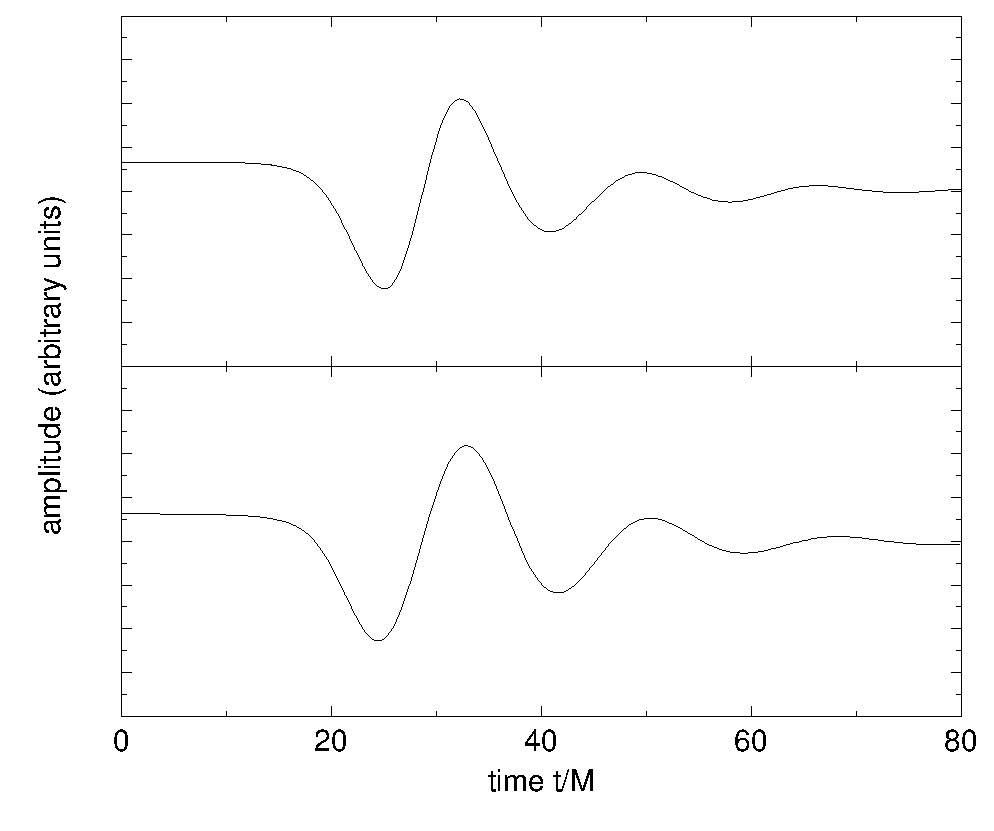
\epsfig{file=Figures/ring-ABW-waveforms.eps,height=2in}
\end{center}
\caption{\label{f:ABWwaveforms}%
  ABW waveforms with $\mu_0=1.9$.}
\end{figure}

These two waveforms correspond to the two codes described in ABW \cite{ABW}, based
on two different set of coordinate systems. To a certain extent, they 
exhibit the limitations of the state of the art in numerical relativity:
both waveforms represent the best effort by correct, ``convergent'' codes,
and yet there is some disagreement among them. This disagreement can be
settled by comparing with the close approximation (see ABW \cite{ABW}). But it is also 
instructive to compare how bad the disagreement is from the point of 
view of a data analyst.

The fitting factor is defined by
\begin{equation}
  \eta = \max_t r(t) = \max_t \alpha^{-1} \Re \int_0^\infty df e^{-2\pi ift}
    \frac{\tilde{a}(f)\tilde{b}^\ast(f)}{S(f)}
\end{equation}
where
\begin{equation}
  \alpha^2 = \int_0^\infty df \frac{\|\tilde{a}(f)\|^2}{S(f)}
    \times\int_0^\infty df \frac{\|\tilde{b}(f)\|^2}{S(f)}
\end{equation}
with $a(t)$ being the close-limit approximation waveform, $b(t)$ being the
ringdown waveform, and $S(f)$ being the detector noise power spectrum.  This
is computed by the program \texttt{corr} (below).  For the LIGO-I
interferometer noise curve and a $200\,M_\odot$ black hole, the fitting
factors are $91\%$ and $85\%$ for the full numerical waveforms.  These
factors represent the fraction of the signal-to-noise ratio that the ringdown
filter will obtain relative to the optimal filter.  As can be seen in the
following figure, the moment at which the ABW \cite{ABW} waveform looks most
``ringdown-like'' is \emph{not} the moment at which the peak signal-to-noise
ratio is obtained.
\begin{figure}[h]
\begin{center}
\index{colorpage}
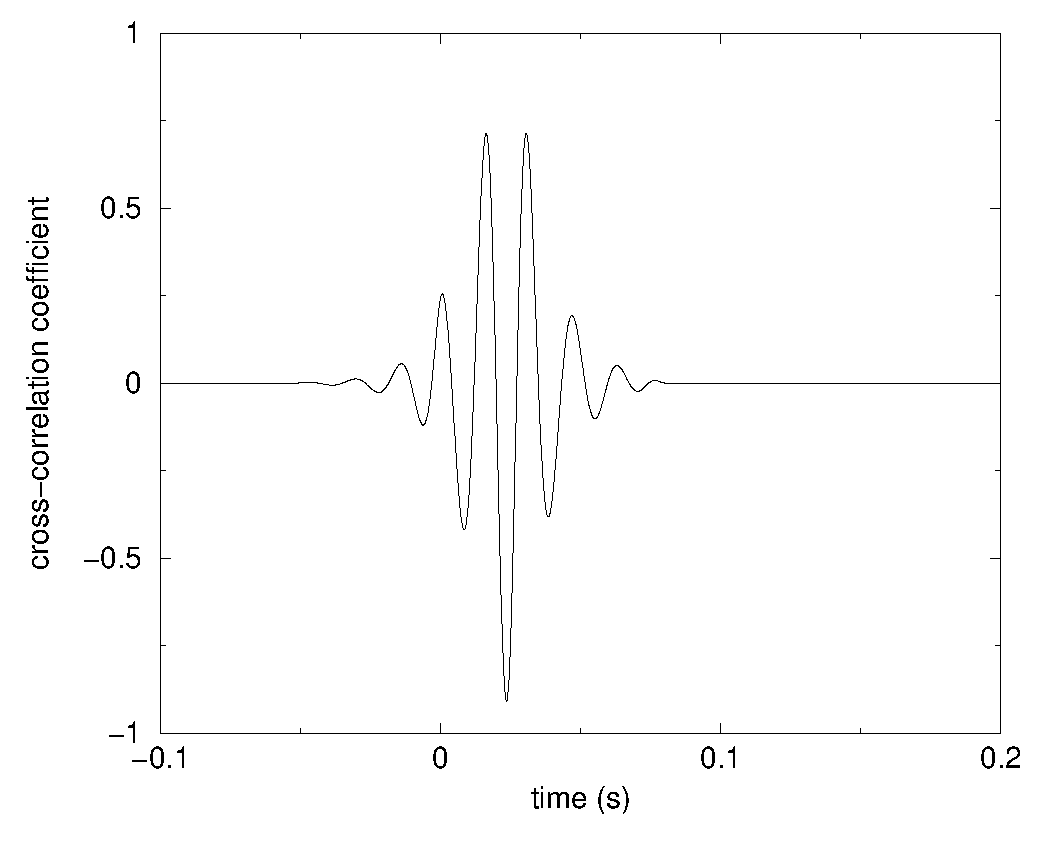
\epsfig{file=Figures/ring-cross-corr2.eps,height=2in}
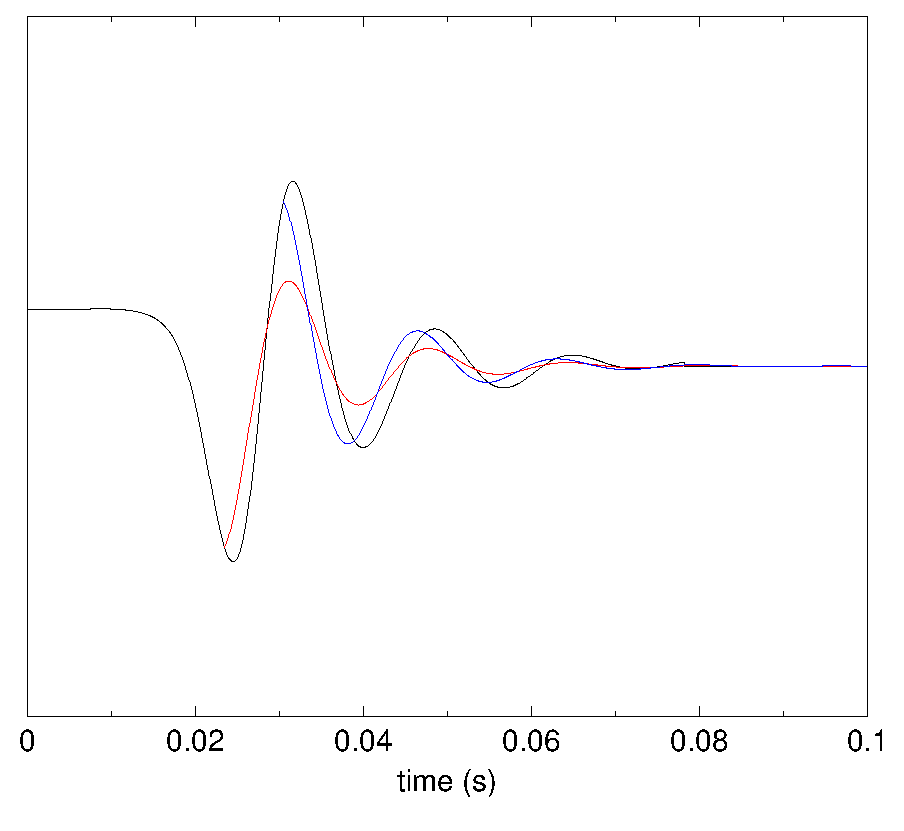
\epsfig{file=Figures/ring-fits2.eps,height=2in}
\end{center}
\caption{\label{f:ABWfits}%
Pure ringdown fits to the ABW waveform.  First: the correlation between the
ABW waveform and a pure ringdown as a function of time.  Second: pure
ringdowns superimposed on the ABW waveform for the times of greatest
correlation.}
\end{figure}

{}From the point of view of source modelling, the difference in head-on
collisions between the full numerical waveforms and the close limit ones
is not substantial.

\begin{description}
\item{Authors:}  Jolien Creighton (jolien@tapir.caltech.edu)
    and Jorge Pullin (pullin@phys.psu.edu)
\end{description}

\clearpage
\subsection{Inspiralling collisions}

For the collision of inspiralling black holes there are no currently
available full numerical simulations. Here the only information
available is from the close limit approximation. In this case, one only
expects to get correctly one portion of the waveform, since in addition
to the final ringdown captured by the close limit approximation, one
also will have the ``chirp'' and ``merger'' phases of the collision.
Nevertheless, it is instructive to see what the use of the ``realistic''
ringdown part of the waveforms yields. The close-limit approximation is
quite limited in validity for inspiralling black hole. The problem is
that for large values of the angular momentum, as are expected in
realistic collisions, the spacetime departs quite radically from that of
a single spinning black holes. Best educated guesses suggest that
trustworthy results from the close limit approximation can only be
obtained up to values of the Kerr parameter of $a=0.5\,M$. At such values,
for separations of a few $M$, the radiated energy is of the order of
$0.3\%$ of the total mass of the system. Of the angular momentum, a
similar fraction gets radiated away. By eyeballing the curve showing the
energy dependence as a function of angular momentum, one could expect
that a ``realistic'' collision with values of $a/M$ close to unity would
probably radiate of the order of $1\%$ of the total mass. This is a
significant extrapolation from the ``reliable'' results, but barring
unexpected physics at the last moments of the collision, it is probably
right. We present here the analysis of a ``close-limit'' type waveform
for the ringdown of the final moments of an inspiralling collision. The
waveform was calculated for $a=0.35\,M$ and separation $L=0.9\,M$
($\mu_0=1.5$).
%We have
%rescaled the amplitude so that $1\%$ of the energy is radiated, as we
%would expect for a realistic collision.
The waveform is shown in
figure~\ref{f:inspiral}.
\begin{figure}
\begin{center} 
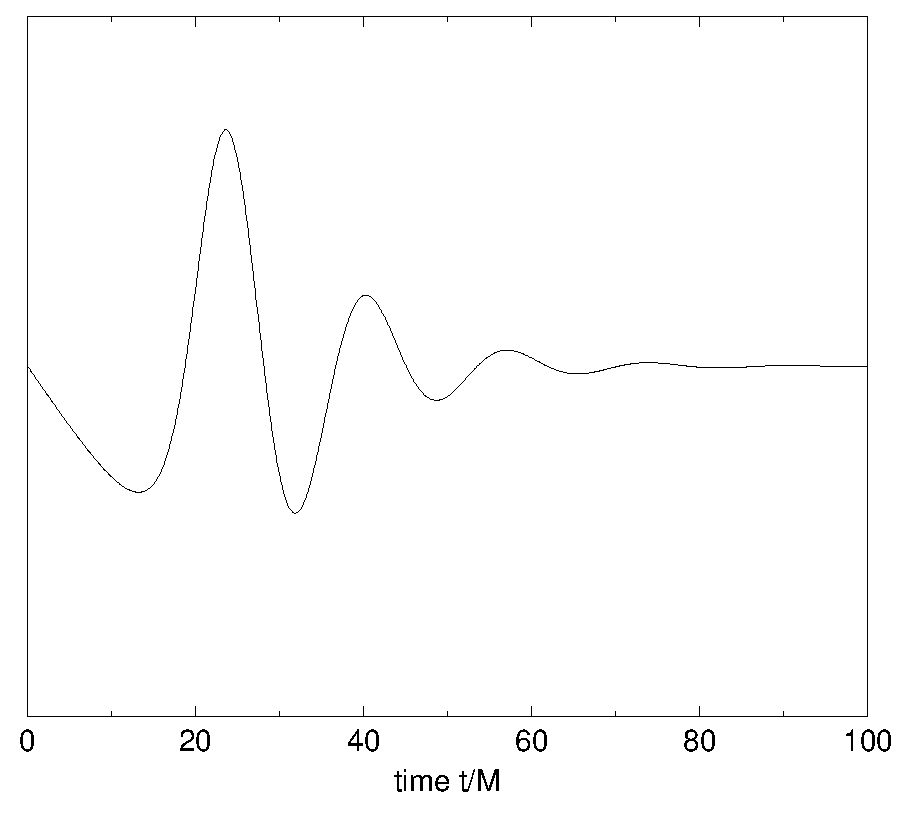
\epsfig{file=Figures/ring-close-insp.eps,height=2in}
\end{center}
\caption{\label{f:inspiral}%
The waveform for the ringdown of an inspiralling collision with
Kerr parameter $a=0.35\,M$ and initial separation $L=0.9\,M$.
%The total
%radiated energy for this case is $E=???/M_{tot}$.
Extrapolations beyond
the realm of validity of the close limit suggest that for a ``realistic''
collision with $a/M$ close to unity about $1\%$ of the mass is radiated.}
\end{figure}

For the LIGO-I noise curve and a total black hole mass of $200\,M_\odot$,
the fitting factor achieved by a quasinormal ringdown template with the
``correct'' $a=0.35\,M$ is $69\%$ (see figure~\ref{f:inspiral-fit}).  However,
this is not a true fitting factor in the sense that the maximization has been
over the time of arrival only---for different values of the ringdown template
mass and spin, the fit will improve.  In particular, only the $\ell=m=2$
quasinormal mode is considered in constructing the ringdown template while the
close-limit waveform contains excitations from the $\ell=2$, $m=0$ as well.
For a rapidly spinning black hole, the $\ell=m=2$ mode will (eventually)
dominate the waveform because it is much longer lived.  However, the spin of
the black hole in the present case is not particularly large, and the $m=0$
mode tends to dominate.  In fact, the fitting factor obtained by using a
ringdown template with $a=0$ is $84\%$---much better than the fit obtained
using the $\ell=m=2$ ringdown with $a=0.35\,M$.  It would be useful to examine
the entire parameter space of quasinormal ringdowns in mass and spin as well
as arrival time in order to obtain the ``true'' fitting factor.

\begin{figure}[h]
\begin{center}
\index{colorpage}
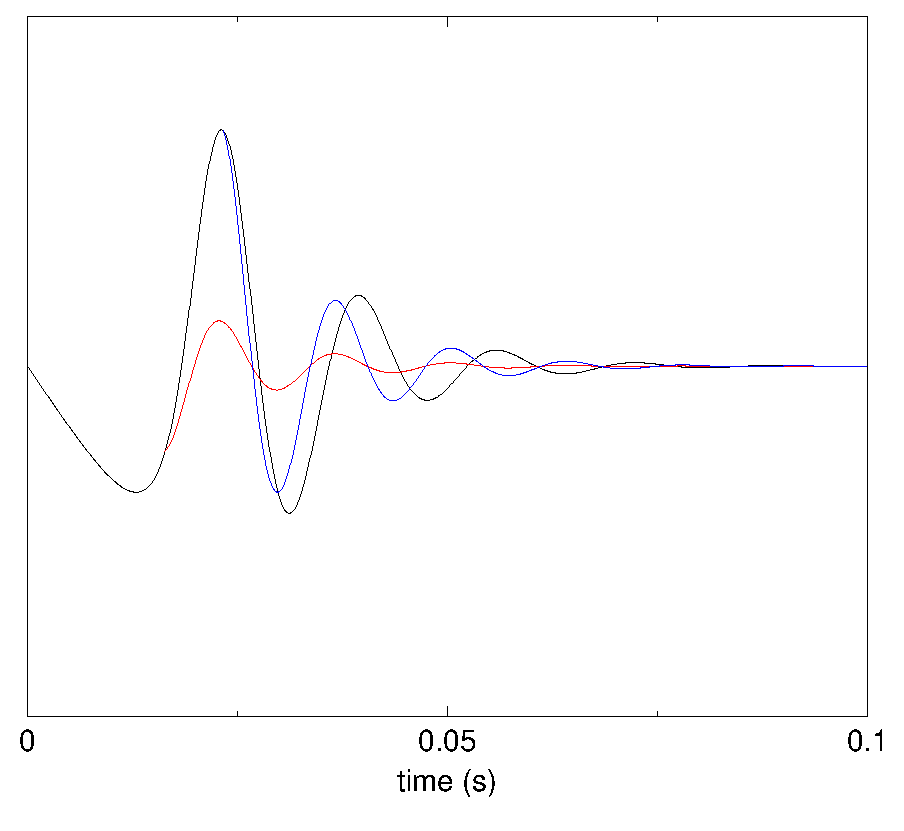
\epsfig{file=Figures/ring-fits-insp.eps,height=2in}
\end{center}
\caption{\label{f:inspiral-fit}%
Pure ringdowns superimposed on the waveform for the ringdown of an
inspiralling collision with Kerr parameter $a=0.35\,M$ and initial separation
$L=0.9\,M$ for the times of greatest correlation.}
\end{figure}

\begin{description}
\item{Authors:}  Jolien Creighton (jolien@tapir.caltech.edu)
    and Jorge Pullin (pullin@phys.psu.edu)
\end{description}

\clearpage
\subsection{Example: \texttt{ring-corr} program}

This program computes the maximum weighted cross-correlation of a black hole
merger waveforms (contained in data files) with ringdown waveforms.  The input
data file(s) contain close-limit approximations or numerical relativity
results for the merger of two black holes.

To execute the program:
\begin{verbatim}
corr [options] [file1 [file2]]
options:
  -h          prints a help message
  -m mass     specifies the black hole mass (in solar masses)
  -s spin     specifies the dimensionless black hole spin [0,1)
  -p powfile  file containing the noise power spectrum
\end{verbatim}
Here, \texttt{file1} and \texttt{file2} are optional filenames containing the
waveform data.  If two arguments are present, the cross-correlations of the
data in the two files is computed; otherwise, the cross-correlation of the
data in the single file (or in file \texttt{close-limit.dat} if there are
no arguments) with a Schwarzschild ringdown is computed.  If a power spectrum
filename is not specified, the program looks for \texttt{ligo-0.dat}.
\lgrindfile{Includes/ring-corr.tex}

\begin{description}
\item{Authors:}  Jolien Creighton (jolien@tapir.caltech.edu)
    and Jorge Pullin (pullin@phys.psu.edu)
\end{description}
